\section{Conversion to Mark}

%----------------------------------------------------------------------
% Cutoffs
%----------------------------------------------------------------------

\subsection{Minimum Distance}

\begin{frame}{Normalized Distance}
\begin{itemize}
\item Need to normalize distances before processing
\end{itemize}
\begin{align*}
\begin{matrix}
\text{Student 1} \\
\text{Student 2} \\
\vdots \\
\text{Student $N$}
\end{matrix}
\hspace{1em}
&
\begin{bmatrix}
    T_{1,1} & T_{1,2} & T_{1,3} & \dots  & T_{1,M} \\
    T_{2,1} & T_{2,2} & T_{2,3} & \dots  & T_{2,M} \\
    \vdots & \vdots & \vdots & \ddots & \vdots \\
    T_{N,1} & T_{N,2} & T_{N,3} & \dots  & T_{N,M}
\end{bmatrix}
\end{align*}
\end{frame}

\note{
\begin{itemize}
\item Now that we have obtained our TED between each pair of student and reference solution, we then need to normalize them before we can move on to computing a final mark
\item Because each reference solution is slightly different, their resulting edit distance to each student will also be slightly different and will be in different ranges
\begin{itemize}
\item For example, reference solution 1 (first column) may range edit distances from 0 to 1000 whereas reference solution $j$ may range from 0 to 600
\end{itemize}
\item As a result, we use normalized each column with the MaxAbsScaler algorithm from the SKLearn library
\begin{itemize}
\item This normalizes each column to be between 0 to 1
\end{itemize}
\end{itemize}
}

%----------------------------------------------------------------------

\subsection{Cutoffs}

\begin{frame}{Cutoffs}
\begin{itemize}
\item Round up our computed score before giving mark back to students
\[
  \text{Mark}_i =
  \begin{cases}
    \text{Score}_i & \text{if Score$_i$ $<$ Cutoff} \\
    100            & \text{if Score$_i$ $\geq$ Cutoff}
  \end{cases}
\]
\item Designated for manual marking if Mark$_i$ is not 100
\item False positive if real mark is $<90$ but scored above cutoff
\end{itemize}
\end{frame}

\note{
\begin{itemize}
\item Before I start dicussing the actual algorithms we used to convert TED into marks, I'll first mention that we actually round up our computed scores before giving the mark back to the student
\item The main reason for this is that our tool does not currently provide meaningful/actionable feedback for the students. Students generally dislike deductions without explainations (or deductions in general!)
\begin{itemize}
\item Minor deductions from TA/our tool are usually small beign errors that are made depending on the marker's mood
\item After rounding up to 100, we say that these full-mark solutions have been automated and leave the rest for manual marking. This is generally fine for courses like ECE459 where most students are expected to receive full marks
\end{itemize}
\item In addition, we say that an automated mark is a false positive if their real mark from human marker (based on historical data) is much lower than their automated mark
\end{itemize}
}

%----------------------------------------------------------------------
% Always Full Marks
%----------------------------------------------------------------------

\subsection{Always Full Marks}

\begin{frame}{Always Full Marks}{Baseline \textquote{automated} approach to compare against}
\begin{center}

\includegraphics[scale=0.6]{presentation/always-full-marks}
\end{center}
\end{frame}

\note{
\begin{itemize}
\item First we need a baseline to compare against
\item The most obvious solution is to simply give everyone a 100. This is an "automated" approach
\end{itemize}
}

%----------------------------------------------------------------------
% Minimum Dist
%----------------------------------------------------------------------

\begin{frame}{Minimum Normalized Distance}
\begin{itemize}
\item Similar solutions should have lower TED
\item Solutions similar to reference solutions get better marks
\end{itemize}
\begin{align*}
\text{Score}_i = 100 \cdot (1 - \min\{ T'_{i,1}, T'_{i,2}, \hdots, T'_{i,M} \})
\end{align*}
\end{frame}

\note{
\begin{itemize}
\item The first approach we tried to combine TED into marks is simply using the minimum distance
\item In my original hypothesis, I said that similar solutions should have lower TED. If a student and reference solution are similar, then they would in theory have low TED
\item This formula is our first attempt at calculating a mark
\begin{itemize}
\item We do 1 minus min TED because the TED are normalized between 0 to 1, 0 being identical to reference solution
\item We multiply by 100 because marks are between 0 to 100
\end{itemize}
\end{itemize}
}

%----------------------------------------------------------------------
% Clustering
%----------------------------------------------------------------------

\subsection{Clustering}

\begin{frame}{Clustering}
\begin{itemize}
\item \textbf{Assume:} unique approaches should have similar features with each other
\item Since most students are expected to receive full marks, most solutions clusters should consist of full marks solutions
\item The volume of full-mark solutions should gravitate the centroid towards \textquote{areas} indicative of correct solutions
\begin{itemize}
\item The closer a student is to the centroid, the higher their mark
\item Score based on parameters of clustering algorithm
\end{itemize}
\end{itemize}
\end{frame}

\note{
\begin{itemize}
\item The next approach we tried was using clustering algorithms like K-Means/Gaussian Mixture/HDBSCAN
\item The basis for this approach is based on the assumption that unique approaches should have similar features with each other (e.g. they might have edit distance of 400 with Ref1, edit distance of 200 with Ref3, etc.)
\item Since most students are expected to receive full marks, most solutions clusters should consist of full marks solutions
\item The volume of full-mark solutions should gravitate the centroid towards \textquote{areas} indicative of correct solutions
\item Therefore, the closer a student is to the centroid of a cluster, the higher their mark
\end{itemize}
}

%----------------------------------------------------------------------

\begin{frame}{K-Means Clustering}{With 4 Clusters}
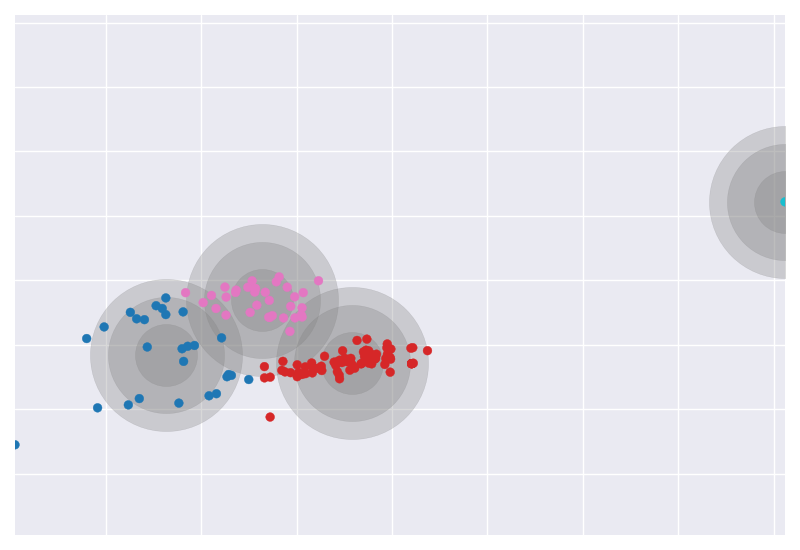
\includegraphics[width=\textwidth]{conversion-to-mark/marking_paster_nbio_ece459-a1-w2017_km}
\end{frame}

\note{
\begin{itemize}
\item That explaination was a bit of a mouthful so now let's take a look at a visual example
\item This graph visualizes the students clustered with K-Means algorithm
\begin{itemize}
\item Each unique color is a unique cluster
\item The concentric circles simply visualizes distance from the centroid
\end{itemize}
\item I dug up the outlier student in the far right
\begin{itemize}
\item Turns out he was the only student in the entire class that used epoll instead of what we told them to use: select or curl multi select (epoll is a newer standard intended to replace select)
\end{itemize}
\end{itemize}
}

%----------------------------------------------------------------------

\begin{frame}{K-Means Clustering}{Full-Marks Highlighted}
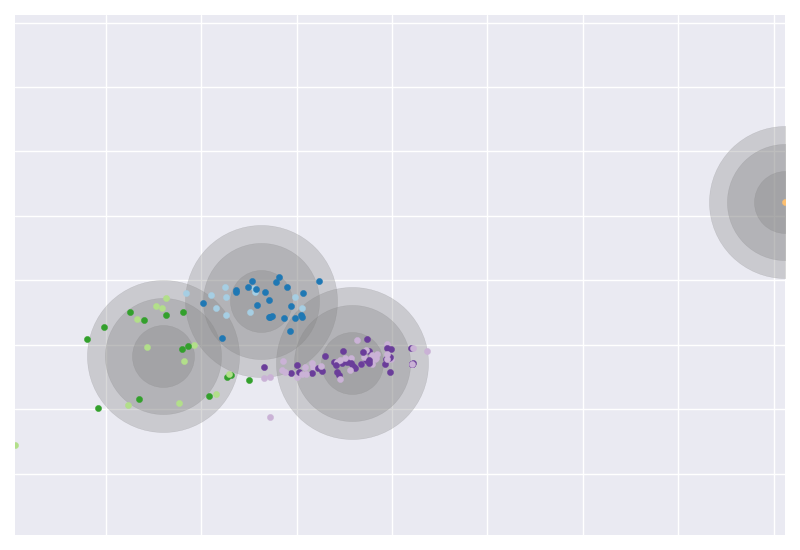
\includegraphics[width=\textwidth]{conversion-to-mark/marking_paster_nbio_ece459-a1-w2017_km_highlight}
\end{frame}

\note{
\begin{itemize}
\item This diagram highlights the students that received full-marks (from human marker) in the darker colors
\item This seems to confirm our hypothesis that clusters' centroid gravitate towards full-mark solutions
\end{itemize}
}

%----------------------------------------------------------------------
% Comparison
%----------------------------------------------------------------------

\subsection{Experimental Results}

\begin{frame}{Experimental Results}
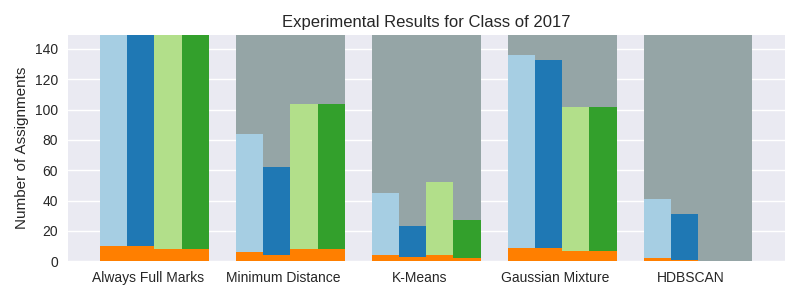
\includegraphics[width=\textwidth]{bar_triple_results_2017_3} \\
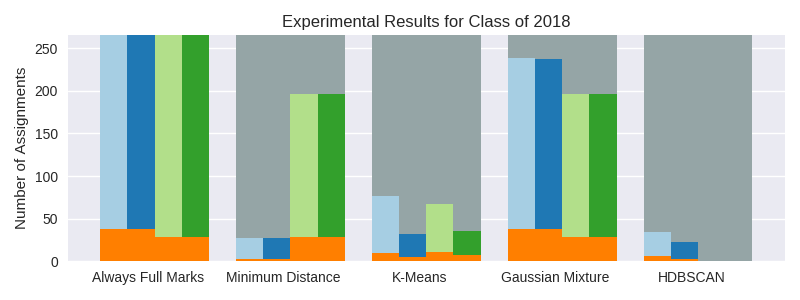
\includegraphics[width=\textwidth]{bar_triple_results_2018_3}
\end{frame}

\note{
\begin{itemize}
\item Finally we can now discuss the experimental results
\begin{itemize}
\item The blue bars represent non-blocking IO solutions; green bars represent pthreads solutions; the darker shade is cutoff at 95, and lighter shade is cutoff at 90
\item The grey bars represent assignments that were automatically graded too low (below cutoffs) and had to be manually marked
\item The orange bars represent the false positives
\end{itemize}
\item
\begin{itemize}
\item We see that K-Means and HDBSCAN are ineffective because their automation rates are too low; then again if we're expecting as many students to receive full marks then they are pretty decent because their false positives are the lowest
\item The MinDist and GM have higher automation rate and false positives; the squashed bars make it look worse than it actually is but regardless the false positive rate is a bit too close to the AlwaysFull
\end{itemize}
\end{itemize}
}

%----------------------------------------------------------------------

\begin{frame}{Shortcomings}{Noise in AST}
\begin{itemize}
\item More edge cases to consider
\item Only looked at correct solutions for clustering features
\end{itemize}
\end{frame}

\note{
\begin{itemize}
\item Clearly our results were not as great as we originally had hoped. As a result, we went back to look at our shortcomings
\item Once we tested our tool with the entire class rather than just a small subset of cases, we found a lot more edge cases to consider
\begin{itemize}
\item For example, there are a few students that wrote their loops to be: while(true) if cond break
\item Had I realized this case eariler, I would have canonicalized loops simply track conditions that break out of them
\end{itemize}
\item Another problem is that we only looked at correct reference solutions for clustering features
\begin{itemize}
\item In a similar related work, the authors mentioned that their false positives went down when their reference solutions also included incorrect solutions
\item Unfortunately since most students are expected to receive full marks, we do not have enough data for "incorrect solutions"
\end{itemize}
\end{itemize}
}

%----------------------------------------------------------------------

\begin{frame}{Shortcomings}{Uncertain ground truth}
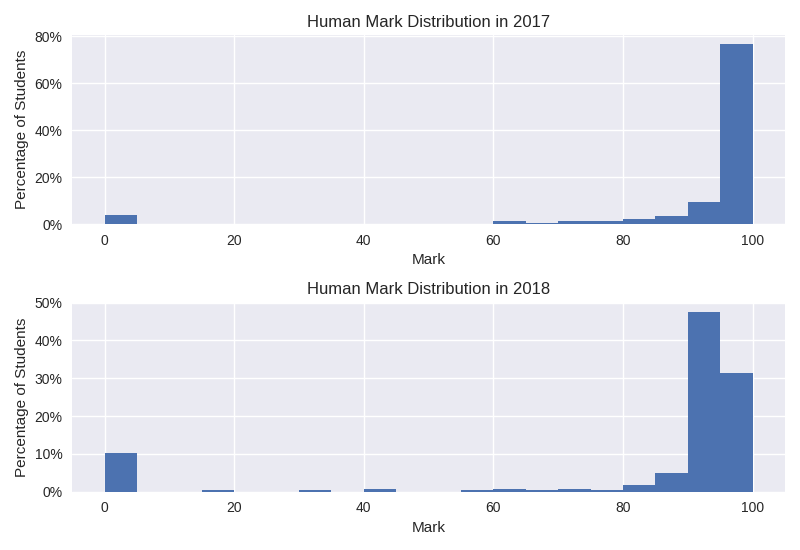
\includegraphics[width=\textwidth]{human_marks}
\end{frame}

\note{
\begin{itemize}
\item Another shortcoming is that we are also uncertain about the validity of our ground truth data
\item We see that there is a discrepency in marker leniency between the 2 classes
\item This brings into question whether human markers are as infallible as we originally assumed
\item Furthermore, we also need to consider that the ground truth mark data includes deductions unrelated to their code: late days deductions, mistakes in their report, etc.
\end{itemize}
}

%----------------------------------------------------------------------

\begin{frame}{Shortcomings}{Uncertain ground truth}
\begin{itemize}
\item Remarked subset of assignments to use as ground-truth
\end{itemize}

\begin{table}
\resizebox{\linewidth}{!}{%
\begin{tabular}{lrrrr} \toprule
\multirow{2}{*}{}
& \multicolumn{2}{c}{2017 Class} & \multicolumn{2}{c}{2018 Class}  \\
& Automated & False Positives & Automated & False Positives  \\
\midrule
Always Full Marks & 20 & 2 & 20 & 7 \\
Min Distance      & 5  & 0 & 1  & 0 \\
K-Means           & 2  & 0 & 2  & 0 \\
Gaussian Mixture  & 8  & 0 & 14 & 3 \\
HDBSCAN           & 0  & - & 0  & - \\
\bottomrule
\end{tabular}
}
\end{table}
\end{frame}

\note{
\begin{itemize}
\item As a result, I've faithfully remarked a subet of assignments to use as ground-truth
\item We see that the automation rate is relatively consistent with our initial result so this is a good random sample
\item We also see that the false positives have significantly dropped with the new ground truth 
\end{itemize}
}
